\documentclass[14pt]{article}

\usepackage{extsizes}
\usepackage{physics}
\usepackage{latexsym} 
\usepackage[left=30mm, top=20mm, right=15mm, bottom=20mm]{geometry}
\usepackage{indentfirst}

%%% Дополнительная работа с математикой
\usepackage{amsmath,amsfonts,amssymb,amsthm,mathtools} % AMS
\usepackage{icomma} % "Умная" запятая: $0,2$ --- число, $0, 2$ 

%%%% Работа с русским языком
\usepackage{cmap}					% поиск в PDF
\usepackage{mathtext} 				% русские буквы в формулах
\usepackage[T2A]{fontenc}			% кодировка
\usepackage[utf8]{inputenc}			% кодировка исходного текста
\usepackage[english,russian]{babel}	% локализация и переносы


%%% Добавлена поддержка для кастомизации таблиц
\usepackage[table,xcdraw]{xcolor}
\usepackage{booktabs}

%%% Работа с картинками
\usepackage{graphicx}  % Для вставки рисунков
\graphicspath{{image/}}  % папки с картинками
\setlength\fboxsep{3pt} % Отступ рамки \fbox{} от рисунка
\setlength\fboxrule{1pt} % Толщина линий рамки \fbox{}
\usepackage{wrapfig} % Обтекание рисунков и таблиц текстом


\usepackage[backend=biber,style=numeric,sorting=none]{biblatex}
\usepackage{csquotes}
%\addbibresource{bibleograf.bib}


\linespread{1.3}
%\pagestyle{plain}

% biber
\usepackage[backend=biber,style=numeric,sorting=none]{biblatex}
\usepackage{csquotes}
\addbibresource{books.bib}

%%%%%%%%%%%%%%%%%%%%%%%%%%%%%%%%%%%%%%%%%%%%%%%%%%%%%%%%%%%%%%%%%%%%%%%%%%%%%%%%%%%%%%%%%%%

\begin{document}
\begin{center}
\small
Федеральное государственное автономное образовательное учреждение высшего образования\\
<<Московский физико-технический институт (Национальный исследовательский университет)>> \\
Физтех-школа аэрокосмических технологий\\
Кафедра вычислительной физики
\end{center}

\begin{flushleft}
\small
\textbf{Направление подготовки:} 03.03.01 Прикладные математика и физика (бакалавриат)\\
\textbf{Направленность(профиль) подготовки:} Вычислительные технологии математического моделирования\\
\end{flushleft}

\begin{center}
\LARGE
\textbf{Исследование компактных схем повышенного порядка точности для численного решения линейного уравнения переноса на нерегулярных сетках}

\small(бакалаврская работа)
\end{center}


\begin{flushright}

\noindent
\textbf{Студент:} \\
Цицварич Йован\\
\underline{\hspace{3cm}}\\
\textbf{Научный руководитель:}\\
Беклемышева Катерина Алексеевна\\
\underline{\hspace{3cm}}\\

\end{flushright}

\begin{center}
\small
Москва\\
2020
\end{center}

\newpage
\section*{Аннотация}
\subsection*{Цели и задачи}

\subsection*{Полученные результаты}

\newpage
\tableofcontents

\newpage
\section*{Используемые обозначения}

\newpage
\section*{Введение}
\addcontentsline{toc}{section}{Введение}
\subsection*{Актуальность темы}


\subsection*{Объект исследования}
В данной задаче мы занимаемся исследованием компактных схем повышенного порядка точности для численного решения линейного уравнения переноса на нерегулярных сетках. Уравнение переноса в однородной постановке имеет вид:
\begin{equation}
u_{t} + \lambda u_{x} = 0,
\label{formula1}
\end{equation} 
где константа $\lambda$ представляет собой скорость переноса.


\subsection*{Значимость исследования.}


\newpage
\section{Теоретические сведения.}
\subsection{Уравнение переноса.}
Уравнение переноса является уравнением в частных производных первого порядка, описывающего изменение величины в пространстве с течением времени. Мы будем заниматься однородным уравнением переноса. Для простоты будем рассматривать случай $\lambda>0$.
\subsection{Граничные условия.}
В данной постановке мы рассматриваем двумерную задачу Коши с периодическими граничными условиями,
\begin{equation}
 \left\lbrace
  \begin{aligned}
    &u_{t} + \lambda u_{x} = 0,  &&x \in [0,1],y \in [0,1], t>0,\\
    &u(x,y,0) = u_0 (x,y), &&x \in [0,1], y \in [0,1].
  \end{aligned} \right.
\end{equation} 
Периодичность граничных условии предполагает замкнутость  пространства по $x$, то есть при достижении правой границы $x = 1$ нашей области $[0, 1]$ происходит перемещение на левую границу $x = 0$ с сохранением значения функции и дальнейшим продолжением ее развития согласно решаемому уравнению. 
Аналитическим решением системы в такой постановке является функция:
\begin{equation}
u(x,y,t) = u(x-\lambda t,y), x \in [0,1], y \in [0,1], t>0.
\end{equation}
\subsection{Сеточно-характеристический метод.}
Классический подход к решению данной задачи предполагает использование разностных схем для аппроксимации частных производных и численного решения уравнения. В данной работе мы  используем сеточно-характеристический подход к решению однородного уравнения переноса. Он заключается в сведении дифференциального уравнения первого порядка в частных производных к обыкновенному дифференциальному уравнению вдоль кривой, называемой характеристикой данного уравнения, такой что:
\begin{equation}
\frac{dx}{dt}=\lambda.
\end{equation}
Вдоль нее уравнение переноса принимает следующий вид:
\begin{equation}
\frac{\partial u}{\partial t} + \frac{dx}{dt} \frac{\partial u}{\partial x}=0 .
\end{equation}
Что равноcильно:
\begin{equation}
\frac{du}{dt}=0.
\end{equation}
То есть вдоль характеристики решение исходного уравнения переноса сохраняется. Используемый нами подход основывается на этом методе – для нахождения значения на $n + 1 - ом$ временном слое следует провести характеристику на $n-ый$ слой по времени и перенести с этого временного слоя значение функции на $n+1-ый$.
\begin{figure}[!h]
\center{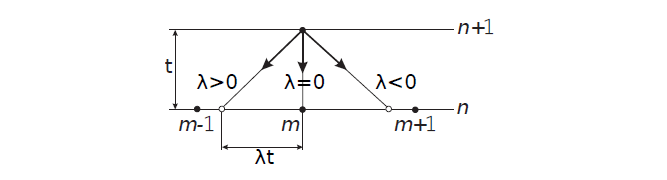
\includegraphics[scale=1]{pics/1.png}}
\caption{Схема сеточно-характеристического метода в одномерном случае на регулярной прямоугольной сетке.}
\label{pic1}
\end{figure}
\subsection{Расчетная сетка.}
 В данной работе рассматривается двумерная задача на нерегулярных треугольных сетках.Нерегулярная треугольная сетка - это разбиение плоскости на неравномерные треугольники. Такие сетки получили широкое примение вместе методе конечных элементов. Их преимущество по сравнению с регулярными сетками заключается в их возможности покрывать комплексные формы, так как единственные накладываемые ограничения при их построении - это максимальная площадь треугольника и его минимальные угол.
\begin{figure}[!h]
\center{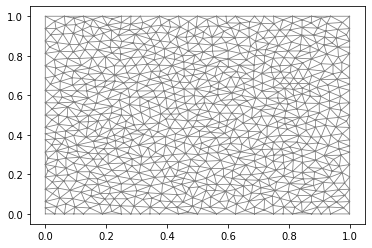
\includegraphics[scale=1]{pics/2.png}}
\caption{Пример используемой расчетной сетки}
\end{figure}
\subsection{Определение точки пересечения характеристики с предыдущим временным слоем.}
В ходе расчета для каждой характеристики, выпущенной из точки на $n+1-ом$ временном слое, по углу наклона, равному $\lambda$ и заданному шагу $\tau$ по времени определяем координату пересечения характеристики с предыдущим временным слоем. Здесь и далее рассматриваем уравнение переноса по переменной x, так как для второй переменной все получается аналогичной последовательностью действии. Алгоритм поиска значении исходной функции $u$ в некоторой точке $(x_{current},y_{current})$, на новом $n+1$ слое по времени состоит в следующем.  Сначала необходимо определить координаты точки пересечения характеристики с $n-ым$ слоем
\begin{equation}
\begin{aligned}
&x_{intersection}=x_{current}- \lambda \tau,\\
&y_{intersection}=y_{current}.
\end{aligned}
\end{equation}

Отдельно стоит выделить случай выпадения точки за область исследования, то есть случай $x_{intersection}<x_{min}$,где $x_{min}=0$ в нашей постановке.  В следствие использования периодических граничных условии, мы сделаем замену 
\begin{equation}
\begin{aligned}
&\widetilde{x}_{intersection}=x_{max}-(x_{min}-x_{intersection} ),\\
&\widetilde{y}_{intersection}=y_{intersection},\\
&где\: x_{max}=1\: в\: нашей\: задаче. 
\end{aligned}
\end{equation}
\subsection{Поиск треугольника.}
После определения координаты пересечения характеристики и временного слоя предстоит определить треугольник, в который характеристика попала. Для этих целей воспользуемся методом известным как метод относительности. Данный метод заключается в том, что при заданной ориентации движения по вершинам треугольника, для каждой стороны вычисляем уравнение прямой и находим по какую сторону от него находится точка, в случае ориентации по часовой – для всех сторон точка будет справа, в случае ориентации против часовой стрелки - слева. Факт нахождения слева или справа определяется по знаку после подстановки координат точки в уравнение прямой.
\begin{figure}[!h!]
\center{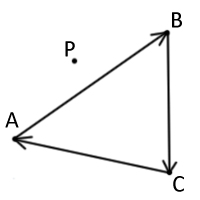
\includegraphics[scale=0.6]{pics/4.png}}
\caption{Ориентация треугольника по часовой.}
\end{figure}
\subsubsection{Оптимизация поиска.}
При измельчении сетки количество треугольников быстро увеличивается и затраты на поиск возрастают. Для оптимизации, так как у нас постоянный шаг по времени $\tau$ и угол наклона характеристик $\lambda$, нам достаточно определить для каждой точки соответствующий ей на предыдущем слое треугольник всего один раз на первом шаге по времени и записать в кэш, далее просто обращаясь к нему по ключу. Так же используется грубый критерий принадлежности треугольнику - треугольник заключается в прямоугольник и по координатам вершин квадрата проводится проверка, попадает точек в данную область или нет. Такой подход помогает избежать многочисленных излишних расчетов и рассчитывать уравнение прямой только для малого количества ближайших треугольников. 
\begin{figure}[!h!]
\center{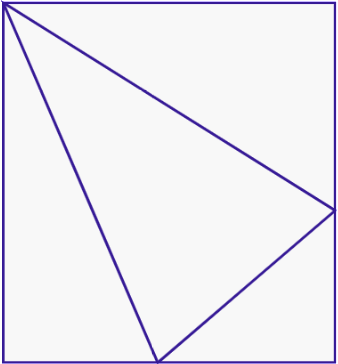
\includegraphics[scale=0.7]{pics/5.png}}
\caption{Пример грубой прямоугольной области для треугольника.}
\end{figure}
\subsection{Интерполяция.}
После определения конкретного треугольника на предыдущем слое по времени, в который попала наша характеристика, нам предстоит определить значение функции в точке пересечения. Для этих целей воспользуемся интерполяционным полиномом первого порядка вида:
\begin{equation}
F(x,y) = ax + by +c, где\: a,b,c \in R
\end{equation} 
Коэффициенты будем искать по значениям функции в вершинах данного треугольника. Имеем систему линейных уравнении:
\begin{equation}
\begin{aligned}[center]
 Ax &= f,\\
где\: А = \begin{pmatrix}
x_1 & y_1 & 1\\
x_2 & y_2 & 1\\
x_3 & y_3 & 1
\end{pmatrix} 
, \: f &= \begin{pmatrix}
f_1 \\
f_2 \\
f_3 
\end{pmatrix},
\: x = \begin{pmatrix}
a \\
b \\
c 
\end{pmatrix},  
\end{aligned}
\end{equation}
где $(x_1,y_1 ),(x_2,y_2 ),(x_3,y_3 )$- координаты вершин исследуемого треугольника, а $f_1,f_2,f_3$- значения функции $u^n$ в соответствующих вершинах. Данная система совместна для любого треугольника, а следовательно, имеет единственное решение. Это свойство следует из того, что
\begin{equation}
detA = x_1(y_2-y_3)-y_1(x_2-x_3)+x_2y_3-x_3y_2,
\end{equation}
данное выражение  не может принимать нулевое значение, так как оно представляет собой подстановку координат вершины $(x_1,y_1)$ в уравнение прямой, связывающей вершины $(x_2,y_2)$ и $(x_3,y_3)$. Равенство нулю означало бы, что точка $(x_1,y_1)$ принадлежит прямой, что противоречит тому, что все три точки являются вершинами одного треугольника. Таким образом, интерполированное значение функции в точке пересечения
\begin{equation}
u_{interpolated}^n=F(x_{intersection},y_{intersection}).
\end{equation}
Данное значение будет вдоль характеристики перенесено на $n+1$ слой по времени в точку $(x_{current},y_{current})$, то есть
$u^{n+1}_i= u_{interpolated}^n$.
По такому алгоритму, проходя по всем точкам сетки, получим значение исходной функции на $n+1$ слое по времени. Данный метод имеет первый порядок сходимости. 
\subsubsection{Повышение порядка.}
Для сеточно-характеристического метода возможно улучшение, если принять в рассмотрение производные исходной функции $u$ и воспользоваться компактной схемой для повышения порядка. Введем функцию производной по $x: \nu(x,y,t)=u_x (x,y,t)$. Здесь и далее рассматривается производная по $x$, случай производной по $y $полностью аналогичен данному. Продифференцируем уравнение переноса для исходной функции $(\ref{formula1})$ по $x$ и получим для функции производной $\nu(x,y,t)$ аналогичное уравнение:
\begin{equation}
\nu_t+\lambda \nu_x=0
\end{equation}
Таким образом, весь описанный раннее алгоритм с интерполяционным полиномом первой степени можно использовать для решения уравнения переноса производных нашей исходной функции. В данном случае меняется подход к интерполяции значения исходной функции на предыдущем слое по времени в точке $(x_{intersection},y_{intersection})$. Так как теперь в каждой вершине треугольника помимо значения исходной функции хранятся значения ее градиента. В таком случае для интерполяционного полинома второго порядка ,
\begin{equation}
\begin{aligned}
P_2 (x,y)=&ax^2+bxy+cy^2+dx+ey+g,\\
&a,b,c,d,e,g \in R.
\end{aligned}
\end{equation}
Для коэффициентов $a,b,c,d,e,g $ имеем систему линейных уравнении
\begin{equation}
\left\lbrace
\begin{aligned}
&ax_1^2+bx_1 y_1+cy_1^2+dx_1+ey_1+g=f_1\\
&ax_2^2+bx_2 y_2+cy_2^2+dx_2+ey_2+g=f_2\\
&ax_3^2+bx_3 y_3+cy_3^2+dx_3+ey_3+g=f_3\\
&2ax_1+by_1+d= f_{1x}'\\
&2ax_2+by_2+d= f_{2x}'\\
&2ax_3+by_3+d= f_{3x}'\\
&bx_1+2cy_1+e= f_{1y}'\\
&bx_2+2cy_2+e= f_{2y}'\\
&bx_3+2cy_3+e= f_{3y}'
\end{aligned},
\right .
\end{equation}
где $f_{ix}',f_{iy}',  \: i=1,2,3\: $--значения производных исходной функции в соответствующих вершинах рассматриваемого треугольника. Первые три уравнения соответствуют значениям функции в вершинах, следующие три значениям производной по переменной $x$ и последние три производной по переменной $y$. Ранг матрицы данной системы линейных уравнен меньше количества уравнении, следовательно система переопределена и не существует точного решения. В данной работе были исследованы два подхода к решению данной проблемы. Первый – из 9 выбрать 6 необходимых уравнении и в случае если система совместна решить ее, в обратном случае взять другие уравнения, второй – чтобы не терять данные о производных функции, можно попытаться решить ее методом наименьших квадратов. Идея данного метода заключается в минимизации нормы разности   $\Vert A\vec{x} - \vec{b}\Vert$, где $А$ – матрица системы линейных уравнении, $\vec{x}$ -- вектор искомых коэффициентов интерполяционного полинома и  $\vec{b}$ -- вектор правых частей нашей системы линейных уравнении. Основным преимуществом такого подхода является гарантированное решение системы линейных уравнении, недостатком же является ограничение на точность накладываемое таким методом, которое может отразиться на точности решения и порядке сходимости. Первый же метод в свою очередь не гарантирует нахождения решения и является намного более ресурсоемким, в худшем случае, при условии, что уравнения на значения исходной функции будут постоянно использоваться в системе, а комбинироваться только уравнения на производные, имеем 20 возможных комбинации, при рассмотрении производных более высокого порядка это число заметно вырастет$\footnote{В случае использования вторых производных для нахождения интерполяционного полинома третьей степени будет существовать 3432 возможных комбинации.}$. В тех случаях, когда ни одна из комбинации уравнении не давала совместной системы, происходит переключение на полином первого порядка, который считается как для исходной функции, так и для ее производных.
\subsection{Расчет порядка.}
В работе проводилось численное исследование порядка сходимости по трем нормам $L_1,\:L_2\: и\: L_{\infty}$, которые задаются следующими формулами:
\begin{equation}
\begin{aligned}
&L_1 =\sum\limits_{i}\frac{\vert u_i^n-U_i^n\vert}{N},\\
&L_2 = \sqrt{\sum\limits_{i}\frac{ (u_i^n-U_i^n)^2}{N^2}},\\
&L_{\infty}=max\vert u_i^n-U_i^n\vert,\\
\end{aligned}
\end{equation}
где $N$-- число точек расчетной сетки, $U$-- проекция аналитического решения на нашу сетку, а $u_i^n$-- значения функции в узлах сетки, полученные в ходе численного расчета с использованием исследуемой схемы. Для расчета порядка сходимости использовались следующие формулы:
\begin{equation}
\begin{aligned}
&p_1 =\frac{\ln \frac{L_1(N_2)}{L_1(N_1)}}{\ln\frac{N_1}{N_2}},\\
&p_2 =\frac{\ln \frac{L_2(N_2)}{L_2(N_1)}}{\ln\frac{N_1}{N_2}},\\
&p_{\infty} =\frac{\ln \frac{L_{\infty}(N_2)}{L_{\infty}(N_1)}}{\ln\frac{N_1}{N_2}},\\
\end{aligned}
\end{equation}
где $N_1\: и\: N_2$ -- число узлов на двух расчетных сетках, при чем $N_1 < N_2$, а $L_1(N_i),\:L_2(N_i)\: и\: L_{\infty}(N_i)$, $i=1,2$  -- значения норм на соответствующих сетках.
\section{Результаты численного эксперимента.}
\subsection{Интерполяция полиномом первого порядка.}
Расчеты проводились для разных типов начального импульса со значением $\lambda$=1. Исследуем порядок сходимости нашей схемы при использовании интерполяционных полиномов первого порядка,для которых как было показано ранее всегда существует единственное решение. Используем следующий вид начального импульса:
\begin{equation}
u(x,y,0) = sin^4(\pi x)sin^4(\pi y).
\end{equation}
В таблицах 1, 2 и 3 приведены результаты расчетов для разных сеток в момент времени $T$=1 и $T$=3 при шаге $\tau=0.01$ и $T$=3 при шаге $\tau=0.001$ соответственно.
\begin{table}[!h!]
\begin{tabular}{|r|r|r|r|r|r|r|}
\hline
\multicolumn{1}{|c|}{N} & \multicolumn{1}{l|}{$L_1$}        & \multicolumn{1}{l|}{$p_1$} & \multicolumn{1}{l|}{$L_2$}     & \multicolumn{1}{l|}{$p_2$} & \multicolumn{1}{l|}{$L_\infty$} & \multicolumn{1}{l|}{$p_\infty$} \\ \hline
280                     & 0,087239                         & -                         & 0,008104                      & \multicolumn{1}{l|}{-}    & 0,561830                    & -                           \\ \hline
336                     & 0,084176                         & 0,196008                  & 0,007179                      & 0,664507                  & 0,552675                    & 0,090111                    \\ \hline
420                     & 0,078477                         & 0,314160                  & 0,006050                      & 0,766924                  & 0,507142                    & 0,385307                    \\ \hline
546                     & 0,071616                         & 0,348732                  & 0,004816                      & 0,869755                  & 0,467492                    & 0,310291                    \\ \hline
833                     & 0,060154                         & 0,412874                  & 0,003341                      & 0,865827                  & 0,406355                    & 0,331795                    \\ \hline
1620                    & 0,042736                         & 0,513982                  & 0,001743                      & 0,978381                  & 0,299077                    & 0,460837                    \\ \hline
2012                    & 0,037003                         & 0,664728                  & 0,001356                      & 1,156000                  & 0,269926                    & 0,473252                    \\ \hline
2691                    & 0,031019                         & 0,606635                  & 0,000990                      & 1,082734                  & 0,227090                    & 0,594256                    \\ \hline
3164                    & 0,026893                         & 0,881299                  & 0,000791                      & 1,385126                  & 0,198694                    & 0,824954                    \\ \hline
3959                    & 0,022135                         & 0,868753                  & 0,000594                      & 1,277442                  & 0,174134                    & 0,588620                    \\ \hline
4553                    & 0,019305    & 0,978573                  & 0,000483                      & 1,478913                  & 0,149670                    & 1,082966                    \\ \hline
5266                    & 0,016754                         & 0,974120                  & 0,000388                      & 1,505377                  & 0,129006                    & 1,021248                    \\ \hline
6347                    & 0,013513                         & 1,151347                  & 0,000287                      & 1,613783                  & 0,104003                    & 1,153835                    \\ \hline
7905                    & 0,010493554 & 1,152088                  & 0,000200                      & 1,640325                  & 0,083046                    & 1,025142                    \\ \hline
10478                   & \multicolumn{1}{l|}{0,007398639} & 1,240195                  & 0,000124                      & 1,713776                  & 0,059363                    & 1,191396                    \\ \hline
15686                   & \multicolumn{1}{l|}{0,005022792} & 0,959898                  & \multicolumn{1}{l|}{6,87E-05} & 1,455265                  & 0,040293                    & 0,960370                    \\ \hline
19665                   & \multicolumn{1}{l|}{0,004150729} & 0,843547                  & \multicolumn{1}{l|}{5,09E-05} & 1,327608                  & 0,033393                    & 0,830886                    \\ \hline
31318                   & 0,002681                         & 0,939637                  & \multicolumn{1}{l|}{2,60E-05} & 1,442039                  & 0,021689                    & 0,927303                    \\ \hline
\end{tabular}
\caption{Результаты расчетов в момент времени Т=1 при $\tau$=0.01}
\end{table}
\newpage
\begin{table}[!h!]
\begin{tabular}{|r|r|r|r|r|r|r|}
\hline
\multicolumn{1}{|l|}{N} & \multicolumn{1}{l|}{$L_1$}        & \multicolumn{1}{l|}{$p_1$} & \multicolumn{1}{l|}{$L_2$}     & \multicolumn{1}{l|}{$p_2$} & \multicolumn{1}{l|}{$L_\infty$} & \multicolumn{1}{l|}{$p_\infty$} \\ \hline
280                     & 0,124177                         & -                         & 0,011289                      & \multicolumn{1}{l|}{-}    & 0,758192                    & -                           \\ \hline
336                     & 0,123780                         & 0,017545                  & 0,010378                      & 0,461467                  & 0,762095                    & -0,028158                   \\ \hline
420                     & 0,122815                         & 0,035079                  & 0,009206                      & 0,537115                  & 0,740077                    & 0,131382                    \\ \hline
546                     & 0,119653                         & 0,099439                  & 0,007757                      & 0,653016                  & 0,710606                    & 0,154882                    \\ \hline
833                     & 0,110048                         & 0,198085                  & 0,005850                      & 0,667990                  & 0,664275                    & 0,159611                    \\ \hline
1620                    & 0,089724                         & 0,306971                  & 0,003462                      & 0,788643                  & 0,566198                    & 0,240176                    \\ \hline
2012                    & 0,081123                         & 0,465016                  & 0,002813                      & 0,957313                  & 0,525163                    & 0,347180                    \\ \hline
2691                    & 0,071354                         & 0,441255                  & 0,002160                      & 0,908072                  & 0,469398                    & 0,386054                    \\ \hline
3164                    & 0,063759                         & 0,695066                  & 0,001785                      & 1,179794                  & 0,428041                    & 0,569599                    \\ \hline
3959                    & 0,054593                         & 0,692393                  & 0,001398                      & 1,089100                  & 0,388150                    & 0,436428                    \\ \hline
4553                    & 0,048725   & 0,813379                  & 0,001169                      & 1,279554                  & 0,349284                    & 0,754732                    \\ \hline
5266                    & 0,043212                         & 0,825343                  & 0,000966                      & 1,310050                  & 0,311220                    & 0,793103                    \\ \hline
6347                    & 0,035855                         & 0,999631                  & 0,000740                      & 1,431530                  & 0,262714                    & 0,907470                    \\ \hline
7905                    & 0,028516316 & 1,043247                  & 0,000532                      & 1,500048                  & 0,215465                    & 0,903214                    \\ \hline
10478                   & 0,020667769 & 1,142375                  & 0,000339                      & 1,595503                  & 0,159360                    & 1,070431                    \\ \hline
15686                   & 0,014362435 & 0,902026                  & 1,94E-04 & 1,387801                  & 0,112091                    & 0,872032                    \\ \hline
19665                   & \multicolumn{1}{l|}{0,011975028} & 0,804137                  & \multicolumn{1}{l|}{1,45E-04} & 1,281201                  & 0,094143                    & 0,771854                    \\ \hline
\end{tabular}
\caption{Результаты расчетов в момент времени Т=3 при $\tau$=0.01}
\end{table}
\newpage
\begin{table}[!h!]
\begin{tabular}{|r|r|r|r|r|r|r|}
\hline
\multicolumn{1}{|l|}{N} & \multicolumn{1}{l|}{$L_1$}        & \multicolumn{1}{l|}{$p_1$} & \multicolumn{1}{l|}{$L_2$}     & \multicolumn{1}{l|}{$p_2$} & \multicolumn{1}{l|}{$L_\infty$} & \multicolumn{1}{l|}{$p_\infty$} \\ \hline
280                     & 0,125539                      & -                         & 0,011425                      & \multicolumn{1}{l|}{-}    & 0,765283                    & -                           \\ \hline
336                     & 0,125780                      & -0,010523                 & 0,010528                      & 0,448274                  & 0,768981                    & -0,026442                   \\ \hline
420                     & 0,125973                      & -0,006868                 & 0,009415                      & 0,500758                  & 0,751386                    & 0,103731                    \\ \hline
546                     & 0,124458                      & 0,046105                  & 0,008043                      & 0,600412                  & 0,728038                    & 0,120314                    \\ \hline
833                     & 0,118458                      & 0,116971                  & 0,006262                      & 0,592555                  & 0,696066                    & 0,106315                    \\ \hline
1620                    & 0,105671                      & 0,171739                  & 0,004021                      & 0,666080                  & 0,629699                    & 0,150647                    \\ \hline
2012                    & 0,099776                      & 0,264908                  & 0,003414                      & 0,754396                  & 0,602648                    & 0,202624                    \\ \hline
2691                    & 0,094210                      & 0,197388                  & 0,002806                      & 0,674784                  & 0,571032                    & 0,185319                    \\ \hline
3164                    & 0,089194                      & 0,337904                  & 0,002447                      & 0,844367                  & 0,542738                    & 0,313839                    \\ \hline
3959                    & 0,083494                      & 0,294604                  & 0,002071                      & 0,745108                  & 0,523187                    & 0,163669                    \\ \hline
4553                    & \multicolumn{1}{l|}{0,080038} & 0,302422                  & 0,001854                      & 0,791496                  & 0,501968                    & 0,296169                    \\ \hline
5266                    & 0,076739                      & 0,289277                  & 0,001655                      & 0,778807                  & 0,482320                    & 0,274454                    \\ \hline
6347                    & 0,072495                      & 0,304746                  & 0,001433                      & 0,772534                  & 0,456291                    & 0,297131                    \\ \hline
7905                    & \multicolumn{1}{l|}{0,066935} & 0,363517                  & 0,001192                      & 0,837687                  & 0,432985                    & 0,238836                    \\ \hline
10478                   & \multicolumn{1}{l|}{0,06037}  & 0,366336                  & 0,000940                      & 0,843923                  & 0,395840                    & 0,318304                    \\ \hline
15686                   & \multicolumn{1}{l|}{0,051561} & 0,390900                  & \multicolumn{1}{l|}{6,64E-04} & 0,861993                  & 0,345194                    & 0,339301                    \\ \hline
19665                   & \multicolumn{1}{l|}{0,046894} & 0,419662                  & \multicolumn{1}{l|}{5,42E-04} & 0,900892                  & 0,317237                    & 0,373586                    \\ \hline
\end{tabular}
\caption{Результаты расчетов в момент времени Т=3 при $\tau$=0.001}
\end{table}

В полученных результатах можно заметить, что порядок сходимости сильно колеблется, одна из предполагаемых причин данного результата может быть особенность треугольной сетки. В следующих таблицах приведены результаты расчетов в момент времени $T$=1 при шаге $\tau=0.01$, но проводилось усреднение результатов - в первом случае по трем близким сеткам, во втором - по пяти.
\begin{table}[]
\begin{tabular}{|l|l|l|l|l|l|l|}
\hline
\multicolumn{1}{|l|}{N} & \multicolumn{1}{l|}{$L_1$}        & \multicolumn{1}{l|}{$p_1$} & \multicolumn{1}{l|}{$L_2$}     & \multicolumn{1}{l|}{$p_2$} & \multicolumn{1}{l|}{$L_\infty$} & \multicolumn{1}{l|}{$p_\infty$} \\ \hline
280,67   & 0,087004 & \multicolumn{1}{r|}{-} & 0,008119 & -        & 0,564257 & \multicolumn{1}{r|}{-} \\ \hline
337,67   & 0,084931 & 0,130451               & 0,007203 & 0,647213 & 0,542017 & 0,217494               \\ \hline
417,00   & 0,078696 & 0,361327               & 0,006117 & 0,774337 & 0,509018 & 0,297659               \\ \hline
552,00   & 0,070055 & 0,414698               & 0,004726 & 0,919789 & 0,462416 & 0,342354               \\ \hline
831,00   & 0,060084 & 0,375316               & 0,003321 & 0,862426 & 0,405557 & 0,320727               \\ \hline
1620,00  & 0,042505 & 0,518484               & 0,001742 & 0,967007 & 0,301624 & 0,443532               \\ \hline
2017,67  & 0,036841 & 0,651520               & 0,001358 & 1,133143 & 0,268957 & 0,522194               \\ \hline
2673,67  & 0,030867 & 0,628502               & 0,000991 & 1,120859 & 0,228014 & 0,586636               \\ \hline
3189,33  & 0,026857 & 0,789079               & 0,000792 & 1,269254 & 0,200701 & 0,723468               \\ \hline
4542,33  & 0,019470 & 0,909602               & 0,000486 & 1,379604 & 0,149425 & 0,834277               \\ \hline
5282,33  & 0,016702 & 1,015741               & 0,000386 & 1,524194 & 0,128056 & 1,022515               \\ \hline
6351,00  & 0,013538 & 1,140012               & 0,000288 & 1,598672 & 0,105007 & 1,077059               \\ \hline
7905,00  & 0,010416 & 1,197904               & 0,000199 & 1,677637 & 0,082589 & 1,097166               \\ \hline
10517,33 & 0,007376 & 1,208484               & 0,000123 & 1,679136 & 0,059359 & 1,156673               \\ \hline
15710,33 & 0,005030 & 0,954019               & 0,000069 & 1,461708 & 0,039952 & 0,986644               \\ \hline
19637,67 & 0,004160 & 0,851554               & 0,000051 & 1,346226 & 0,033361 & 0,807956               \\ \hline
19635,4  & 0,004156 & 0,840542               & 0,000051 & 1,341001 & 0,033315 & 0,804780               \\ \hline
\end{tabular}
\caption{Результаты расчетов с усреднением по трем сеткам в момент времени Т=1 при $\tau$=0.01}
\end{table}
\newpage
\begin{table}[]
\begin{tabular}{|l|l|l|l|l|l|l|}
\hline
\multicolumn{1}{|l|}{N} & \multicolumn{1}{l|}{$L_1$}        & \multicolumn{1}{l|}{$p_1$} & \multicolumn{1}{l|}{$L_2$}     & \multicolumn{1}{l|}{$p_2$} & \multicolumn{1}{l|}{$L_\infty$} & \multicolumn{1}{l|}{$p_\infty$} \\ \hline
279,6   & 0,087344 & \multicolumn{1}{r|}{-} & 0,008184 & -        & 0,564051 & \multicolumn{1}{r|}{-} \\ \hline
337,8   & 0,084591 & 0,169375               & 0,007184 & 0,689360 & 0,535931 & 0,270446               \\ \hline
416,4   & 0,079015 & 0,325980               & 0,006154 & 0,739578 & 0,510326 & 0,234019               \\ \hline
551,6   & 0,070695 & 0,395698               & 0,004773 & 0,903919 & 0,464915 & 0,331451               \\ \hline
830,0   & 0,059773 & 0,410718               & 0,003318 & 0,890034 & 0,406939 & 0,325963               \\ \hline
1621,2  & 0,042415 & 0,512414               & 0,001732 & 0,970793 & 0,300838 & 0,451226               \\ \hline
2022,8  & 0,036736 & 0,649400               & 0,001353 & 1,117538 & 0,268596 & 0,512214               \\ \hline
2666,0  & 0,030803 & 0,638020               & 0,000991 & 1,125838 & 0,227518 & 0,601167               \\ \hline
3191,0  & 0,026830 & 0,768294               & 0,000793 & 1,243695 & 0,200704 & 0,697596               \\ \hline
3966,2  & 0,022054 & 0,901355               & 0,000587 & 1,379341 & 0,169203 & 0,785066               \\ \hline
4542,8  & 0,019476 & 0,915915               & 0,000486 & 1,399589 & 0,149133 & 0,930224               \\ \hline
5287,2  & 0,016665 & 1,026987               & 0,000386 & 1,508776 & 0,128601 & 0,976122               \\ \hline
6351,2  & 0,013555 & 1,126755               & 0,000288 & 1,592881 & 0,105564 & 1,076610               \\ \hline
7895,4  & 0,010377 & 1,227542               & 0,000199 & 1,714125 & 0,081532 & 1,186937               \\ \hline
10521,4 & 0,007362 & 1,195622               & 0,000123 & 1,668186 & 0,059174 & 1,116228               \\ \hline
15699,6 & 0,005015 & 0,958838               & 0,000068 & 1,464709 & 0,039887 & 0,985561               \\ \hline
19635,4 & 0,004156 & 0,840542               & 0,000051 & 1,341001 & 0,033315 & 0,804780               \\ \hline
\end{tabular}
\caption{Результаты расчетов с усреднением по пяти сеткам в момент времени Т=1 при $\tau$=0.01}
\end{table}
Заметного результата усреднение не дало - порядок сходимости и дальше колеблется. На рисунке 5 можно увидеть вид численного решения на разных сетках.
\begin{figure}[!h!]
\center{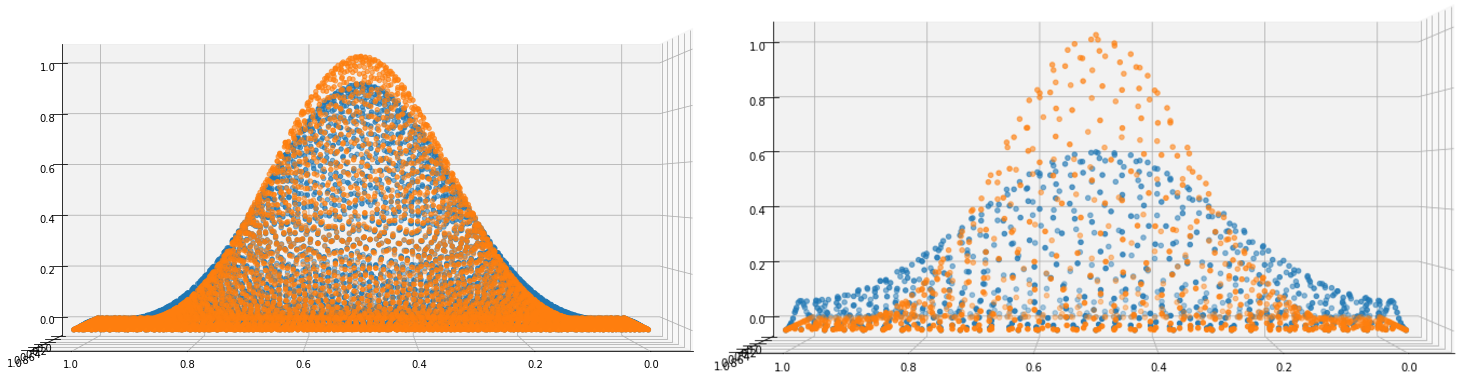
\includegraphics[scale=0.35]{pics/6.png}}
\caption{Результаты расчета на сетках с разным числом расчетных узлов. Слева - 6347 узлов, справа - 833. Синим изображено численное решение, оранжевым аналитическое в момент времени Т=1 при шаге $\tau$=0.01.}
\end{figure}
\newpage
\subsection{Интерполяция полиномом второго порядка.}
Далее проведем расчеты с использованием производных для повышения порядка полинома с начальным импульсом вида:
\begin{equation}
\left\lbrace
\begin{aligned}
&u(x,y,0) = sin^4(\pi x)sin^4(\pi y),\\
&u_x(x,y,0) =  4\pi sin^3(\pi x) sin^4(\pi y)  cos(\pi x),\\
&u_y(x,y,0) = 4\pi sin^4(\pi x)sin^3(\pi y)cos(\pi y).
\end{aligned}
\right .
\end{equation}
На рисунке 6 представлены результаты численных расчетов в сравнении с проекцией аналитического решения на расчетную сетку.
\begin{figure}[!h!]
\center{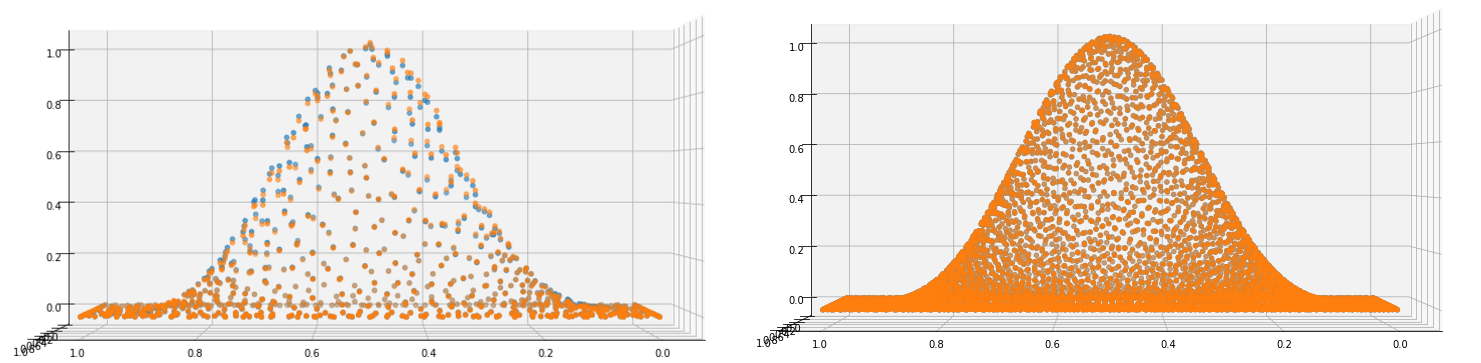
\includegraphics[scale=0.35]{pics/7.png}}
\caption{Результаты расчета на сетках с разным числом расчетных узлов. Слева - 833 узлов, справа - 6347. Синим изображено численное решение, оранжевым аналитическое в момент времени Т=1 при шаге $\tau$=0.01.}
\end{figure}
 В таблице 7 представлены усредненные расчеты по трем сеткам с близким количеством узлов.
\begin{table}[h]
\begin{tabular}{|r|r|r|r|r|r|r|}
\hline
\multicolumn{1}{|l|}{N} & \multicolumn{1}{l|}{$L_1$}        & \multicolumn{1}{l|}{$p_1$} & \multicolumn{1}{l|}{$L_2$}     & \multicolumn{1}{l|}{$p_2$} & \multicolumn{1}{l|}{$L_\infty$} & \multicolumn{1}{l|}{$p_\infty$} \\ \hline
280                         & 0,014964                      & -                         & 1,512E-03                      & \multicolumn{1}{l|}{-}    & 0,097890                      & -                           \\ \hline
336                         & 0,012229                      & 1,106800                  & 1,138E-03                      & 1,562403                  & 0,083861                      & 0,848404                    \\ \hline
420                         & 0,009685                      & 1,045366                  & 7,805E-04                      & 1,688373                  & 0,059121                      & 1,566609                    \\ \hline
546                         & 0,006429                      & 1,561802                  & 4,697E-04                      & 1,935249                  & 0,041508                      & 1,348090                    \\ \hline
833                         & 0,003259                      & 1,608495                  & 1,936E-04                      & 2,098861                  & 0,022847                      & 1,413438                    \\ \hline
1620                        & 0,001042                      & 1,713681                  & 4,271E-05                      & 2,271903                  & 0,006554                      & 1,877473                    \\ \hline
2012                        & 0,000630                      & 2,321321                  & 2,381E-05                      & 2,696059                  & 0,004532                      & 1,702130                    \\ \hline
2691                        & 0,000320                      & 2,335319                  & 9,757E-06                      & 3,068269                  & 0,002330                      & 2,288513                    \\ \hline
3164                        & 0,000182                      & 3,465536                  & 5,015E-06                      & 4,110660                  & 0,001360                      & 3,322698                    \\ \hline
3959                        & 0,000111                      & 2,202140                  & 2,625E-06                      & 2,887269                  & 0,000675                      & 3,127833                    \\ \hline
4553                        & \multicolumn{1}{l|}{0,000108} & 0,196558                  & 2,383E-06                      & 0,693333                  & 0,000633                      & 0,457131                    \\ \hline
5266                        & 0,000112                      & -0,229490                 & 2,428E-06                      & -0,130072                 & 0,000750                      & -1,168079                   \\ \hline
6347                        & 0,000092                      & 1,062375                  & 1,839E-06                      & 1,489868                  & 0,000574                      & 1,436844                    \\ \hline
\multicolumn{1}{|l|}{7905}  & \multicolumn{1}{l|}{0,000062} & 1,788875                  & \multicolumn{1}{l|}{1,131E-06} & 2,214683                  & \multicolumn{1}{l|}{0,000414} & 1,488286                    \\ \hline
\multicolumn{1}{|l|}{10478} & \multicolumn{1}{l|}{0,000021} & 3,900467                  & \multicolumn{1}{l|}{3,119E-07} & 4,570369                  & \multicolumn{1}{l|}{0,000148} & 3,655011                    \\ \hline
\multicolumn{1}{|l|}{15686} & \multicolumn{1}{l|}{0,000009} & 2,053784                  & \multicolumn{1}{l|}{1,147E-07} & 2,479577                  & \multicolumn{1}{l|}{0,000071} & 1,821542                    \\ \hline
\multicolumn{1}{|l|}{19665} & \multicolumn{1}{l|}{0,000006} & 1,621655                  & \multicolumn{1}{l|}{6,890E-08} & 2,254299                  & \multicolumn{1}{l|}{0,000053} & 1,315016                    \\ \hline
\end{tabular}
\caption{Результаты расчетов c полиномом второго порядка в момент времени Т=1 при $\tau$=0.01}
\end{table}
\begin{table}[]
\begin{tabular}{|l|l|l|l|l|l|l|}
\hline
\multicolumn{1}{|l|}{N} & \multicolumn{1}{l|}{$L_1$}        & \multicolumn{1}{l|}{$p_1$} & \multicolumn{1}{l|}{$L_2$}     & \multicolumn{1}{l|}{$p_2$} & \multicolumn{1}{l|}{$L_\infty$} & \multicolumn{1}{l|}{$p_\infty$} \\ \hline
280,6667 & 0,014778 & \multicolumn{1}{r|}{-} & 1,519E-03 & -        & 0,099051 & \multicolumn{1}{r|}{-} \\ \hline
337,6667 & 0,012131 & 1,067443               & 1,114E-03 & 1,676752 & 0,078014 & 1,291294               \\ \hline
417      & 0,009278 & 1,270688               & 7,566E-04 & 1,833995 & 0,056906 & 1,494970               \\ \hline
552      & 0,006295 & 1,383038               & 4,524E-04 & 1,834084 & 0,039655 & 1,287842               \\ \hline
831      & 0,003358 & 1,536348               & 1,966E-04 & 2,037467 & 0,022470 & 1,388535               \\ \hline
1620     & 0,001052 & 1,738829               & 4,362E-05 & 2,255085 & 0,007042 & 1,738115               \\ \hline
2017,667 & 0,000626 & 2,363366               & 2,309E-05 & 2,897314 & 0,004329 & 2,216993               \\ \hline
2673,667 & 0,000315 & 2,441933               & 1,002E-05 & 2,965788 & 0,002418 & 2,069100               \\ \hline
3189,333 & 0,000175 & 3,325044               & 4,829E-06 & 4,140053 & 0,001234 & 3,813001               \\ \hline
3959,333 & 0,000110 & 2,145818               & 2,565E-06 & 2,925749 & 0,000655 & 2,927741               \\ \hline
4542,333 & 0,000107 & 0,182882               & 2,390E-06 & 0,513785 & 0,000663 & -0,091470              \\ \hline
5282,333 & 0,000110 & -0,181310              & 2,381E-06 & 0,023717 & 0,000711 & -0,461124              \\ \hline
6351     & 0,000093 & 0,923076               & 1,867E-06 & 1,321988 & 0,000600 & 0,918882               \\ \hline
7905     & 0,000061 & 1,897085               & 1,113E-06 & 2,363004 & 0,000408 & 1,765003               \\ \hline
10517,33 & 0,000019 & 4,154734               & 2,863E-07 & 4,754753 & 0,000138 & 3,804645               \\ \hline
15710,33 & 0,000009 & 1,787046               & 1,158E-07 & 2,254658 & 0,000070 & 1,668703               \\ \hline
19637,67 & 0,000006 & 1,576792               & 7,230E-08 & 2,112624 & 0,000055 & 1,136076               \\ \hline
\end{tabular}
\caption{Результаты усреднения расчетов по трем сеткам c полиномом второго порядка в момент времени Т=1 при $\tau$=0.01}
\end{table}

\end{document}
